\subsection{Spatial Decision Support}
\label{sec:spatial_decision_support}
%Investigating and making decisions using only the heatmap without any supplementary information are demanding and hard to unserstand the actual events.
In Section~\ref{sec:spatial_analysis}, we introduced our spatial analysis to explore the Twitter user distribution.
In addition to the analysis, our system allows the analysts to utilize supplementary information in order to support understanding of the situations and decision-making in disaster management.
The spatial characteristics together with heterogeneous information can assist in disaster management and migrating hazards where the problems have spatial components~\cite{Andrienko:2007:GAS}.
The supplementary information can be various types of infrastructures (i.e., school, park, supermarket, and shelter), as well as spatial information of disaster events (i.e., hurricane path and damage area of a tornado).
In this section, we describe how our system supports spatial decision-making by correlating such spatial information with location-based microblog data.

\subsubsection{Infrastructure Data}
\label{sec:infrastructure_data}
%
During a natural disaster event, such as Hurricane Sandy, analysts would assume that many people might want to go to the supermarket before staying or evacuating, but they would need supporting evidence before making appropriate decisions and plans.
With our system support, the analysts can simply overlay the locations of large supermarkets on the heatmap of the Twitter user distribution.
The infrastructure locations are indicated by standard symbols~\cite{Robinson:2012:DMS} as 
shown on the right side of Figure~\ref{fig:heatmap_manhattan}.
%presented in Figure~\ref{fig:symbols}.
%(e.g., \textit{Trader Joe's} and \textit{Whole Foods Market}).
%Note that there is no major retail chains, such as Walmart and Target in Manhattan.
A relatively large number of people immediately went to supermarkets nearby the evacuation area, instead of the emergency shelter as shown in Figure~\ref{fig:heatmap_manhattan} (Right).
However, October 28th was Sunday and many people generally would go for grocery shopping on Saturday or Sunday; therefore, the analysts might need to verify whether the heatmap shown in the figure is a normal periodic situation.
The analysts can investigate new Twitter user distributions for different time frames by simply manipulating the time context.
In Figure~\ref{fig:heatmap_manhattan} (Left and Center), we show two distributions for one and two weeks before the disaster period respectively.
Here, we see that the hotspot locations are very different from the ones for October 28th shown in Figure~\ref{fig:heatmap_manhattan} (Right).
For further analysis, we can explore another popular Sunday location\textemdash large parks\textemdash by superimposing the locations on each heatmap.
%, since we can expect that parks would be populated on Sunday.
As shown in Figure~\ref{fig:heatmap_manhattan} (Left and Center), many hotspots overlap with the park areas in normal situations.
Therefore, we can conclude that the situation on October 28th is an unusual non-periodic pattern.
%
%This system can support the analysts to understand the unusual movement patterns and plan resource allocation accordingly for such emergency events.
%
%can realize that the situation on October 28th is unusual and non-periodic. 
%This system can support them to make plans for preparing some responses for the emergency events.



\subsubsection{Disaster Event Data}
\label{sec:event_data}
%
In Section~\ref{sec:infrastructure_data}, we explained how the infrastructure data help the analysts to understand and examine the emergent situations.
During severe weather conditions, people tend to be sensitive to the dynamic variance of the weather conditions.
Relationship analysis, therefore, between the public responses and the spatiotemporal pattern of the severe weather is important.
Our system overlays geographic information of disaster events, for example, center positions and tracks of a hurricane, and damaged areas by a tornado, in order to provide further analysis.
Two case studies are presented as follows:

\textbf{Track of Hurricane:} Figure~\ref{fig:east_coast}~(1) and (2) show the southeastern coast areas of the United States, whereas,
Figure~\ref{fig:east_coast}~(3), (4), and (5) show the northeastern coast areas.
In the figures the distributions of Twitter users for each consecutive date, from October 26th to 30th, 2012, are presented 
using the heatmap visualizations.
We use the number of Twitter users who posted Twitter messages containing one of the following keywords: \textit{hurricane, storm}, and \textit{sandy} in order to analyze Tweets that are highly related to Hurricane Sandy.
Note that Hurricane Sandy reached the southeastern Florida coast on October 26th and passed, then, over the northeastern coast on October 30th, 2012~\cite{WKP:2012:SANDY}.
As shown in Figure~\ref{fig:east_coast}, our system is able to overlay the track of the hurricane on the map.
% according to a time period of interest.
%(the texts on the map were manually added).
The blue pins and the blue lines represent the center locations of the hurricane and its path respectively.

\begin{figure}[tbh]
\centering
%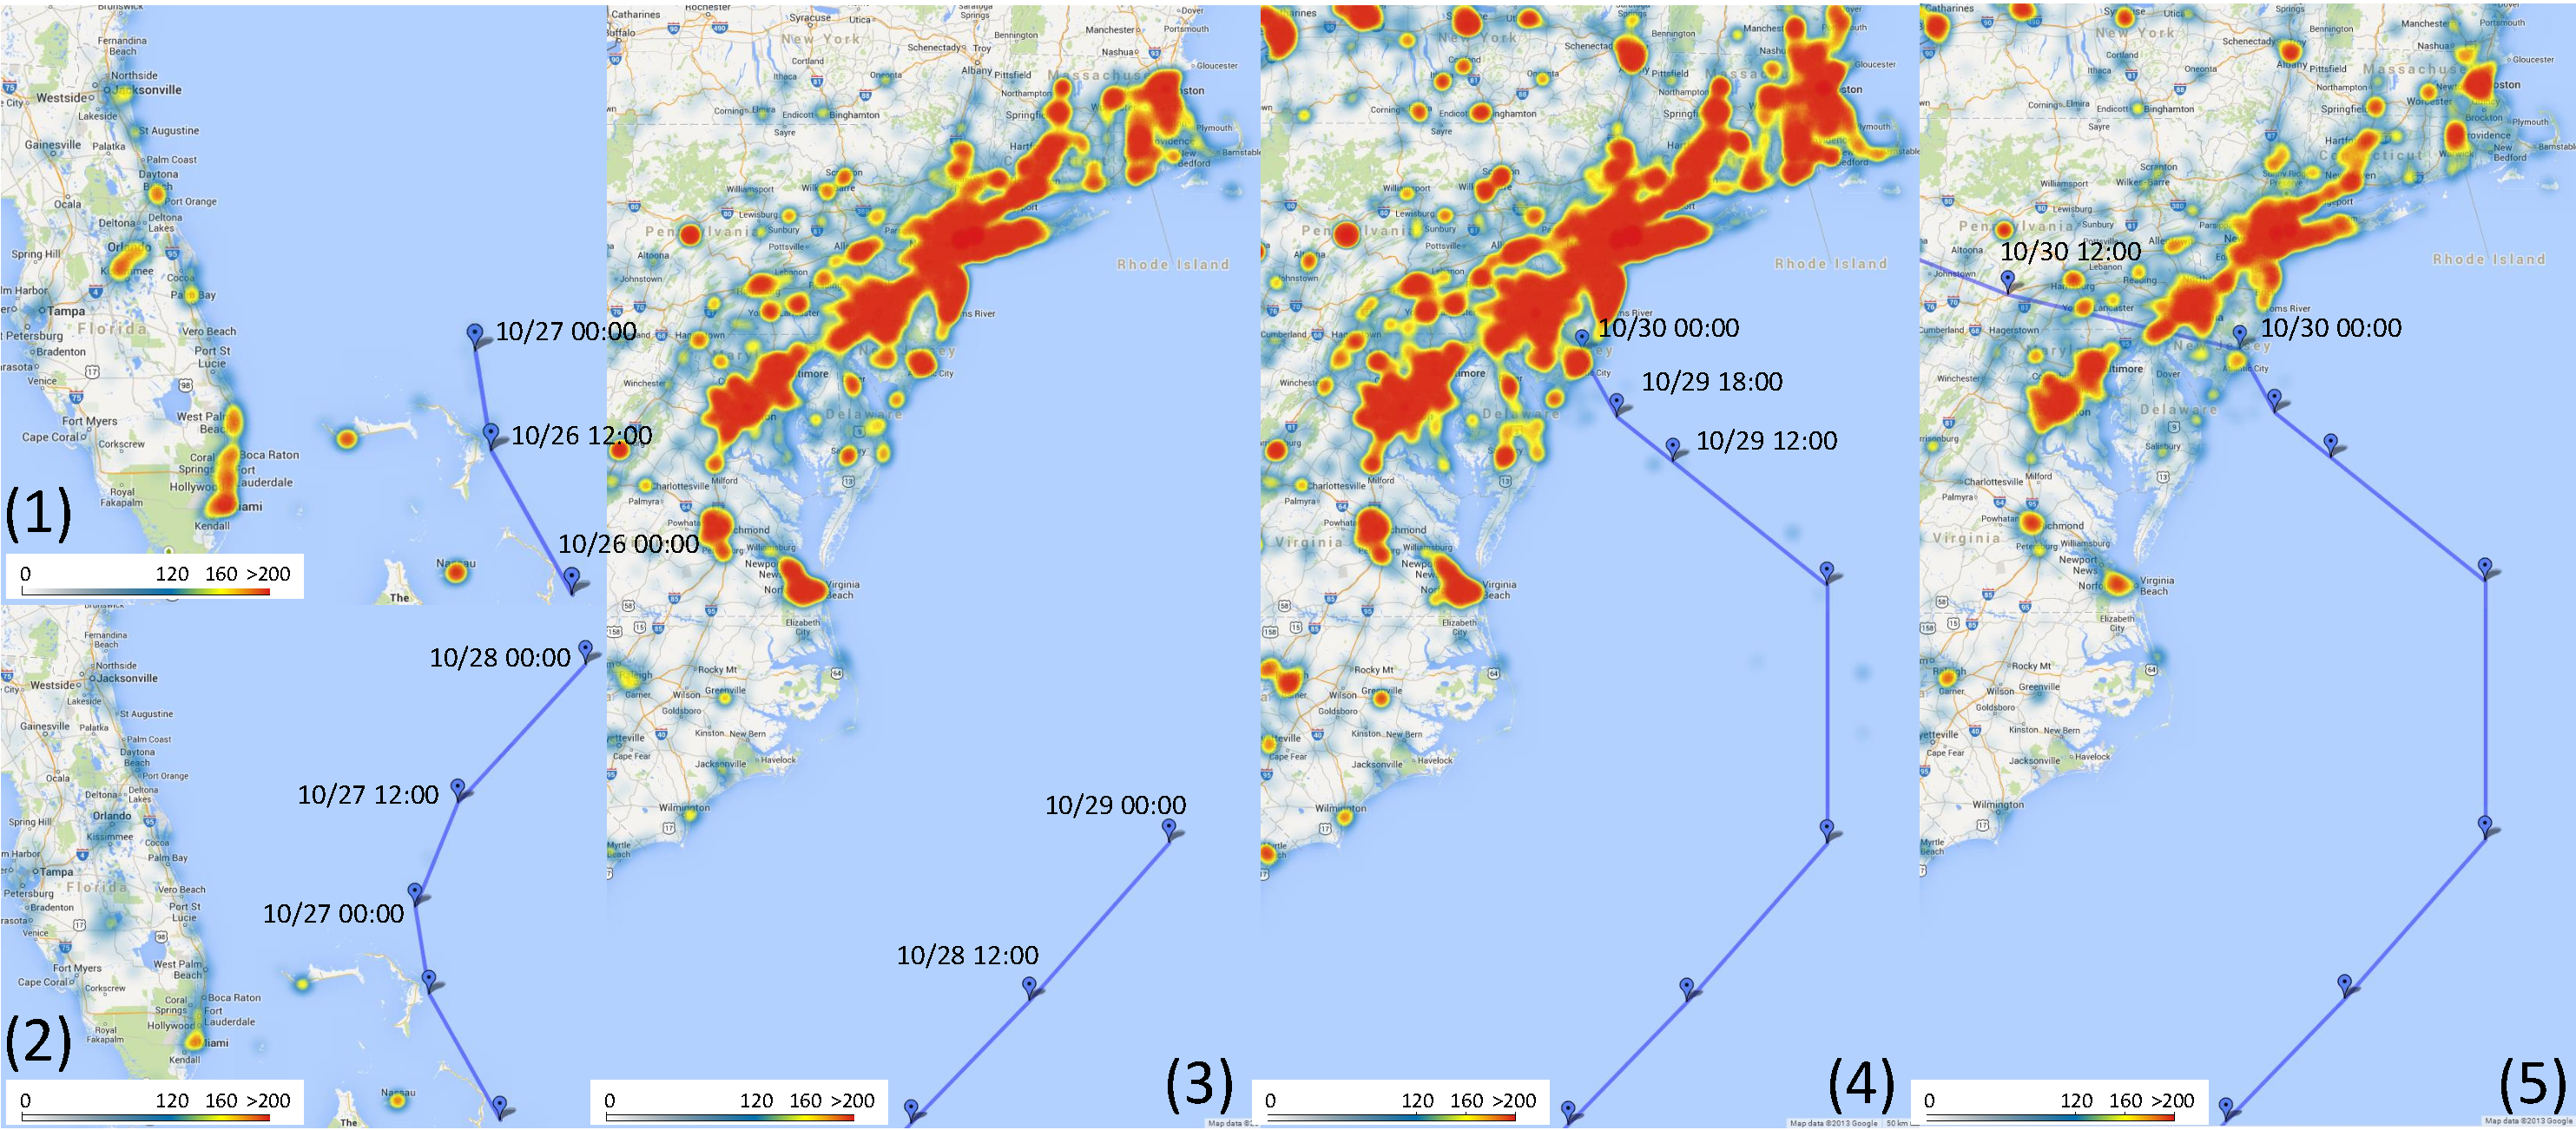
\includegraphics[width=0.85\linewidth]{East_Coast_v7}
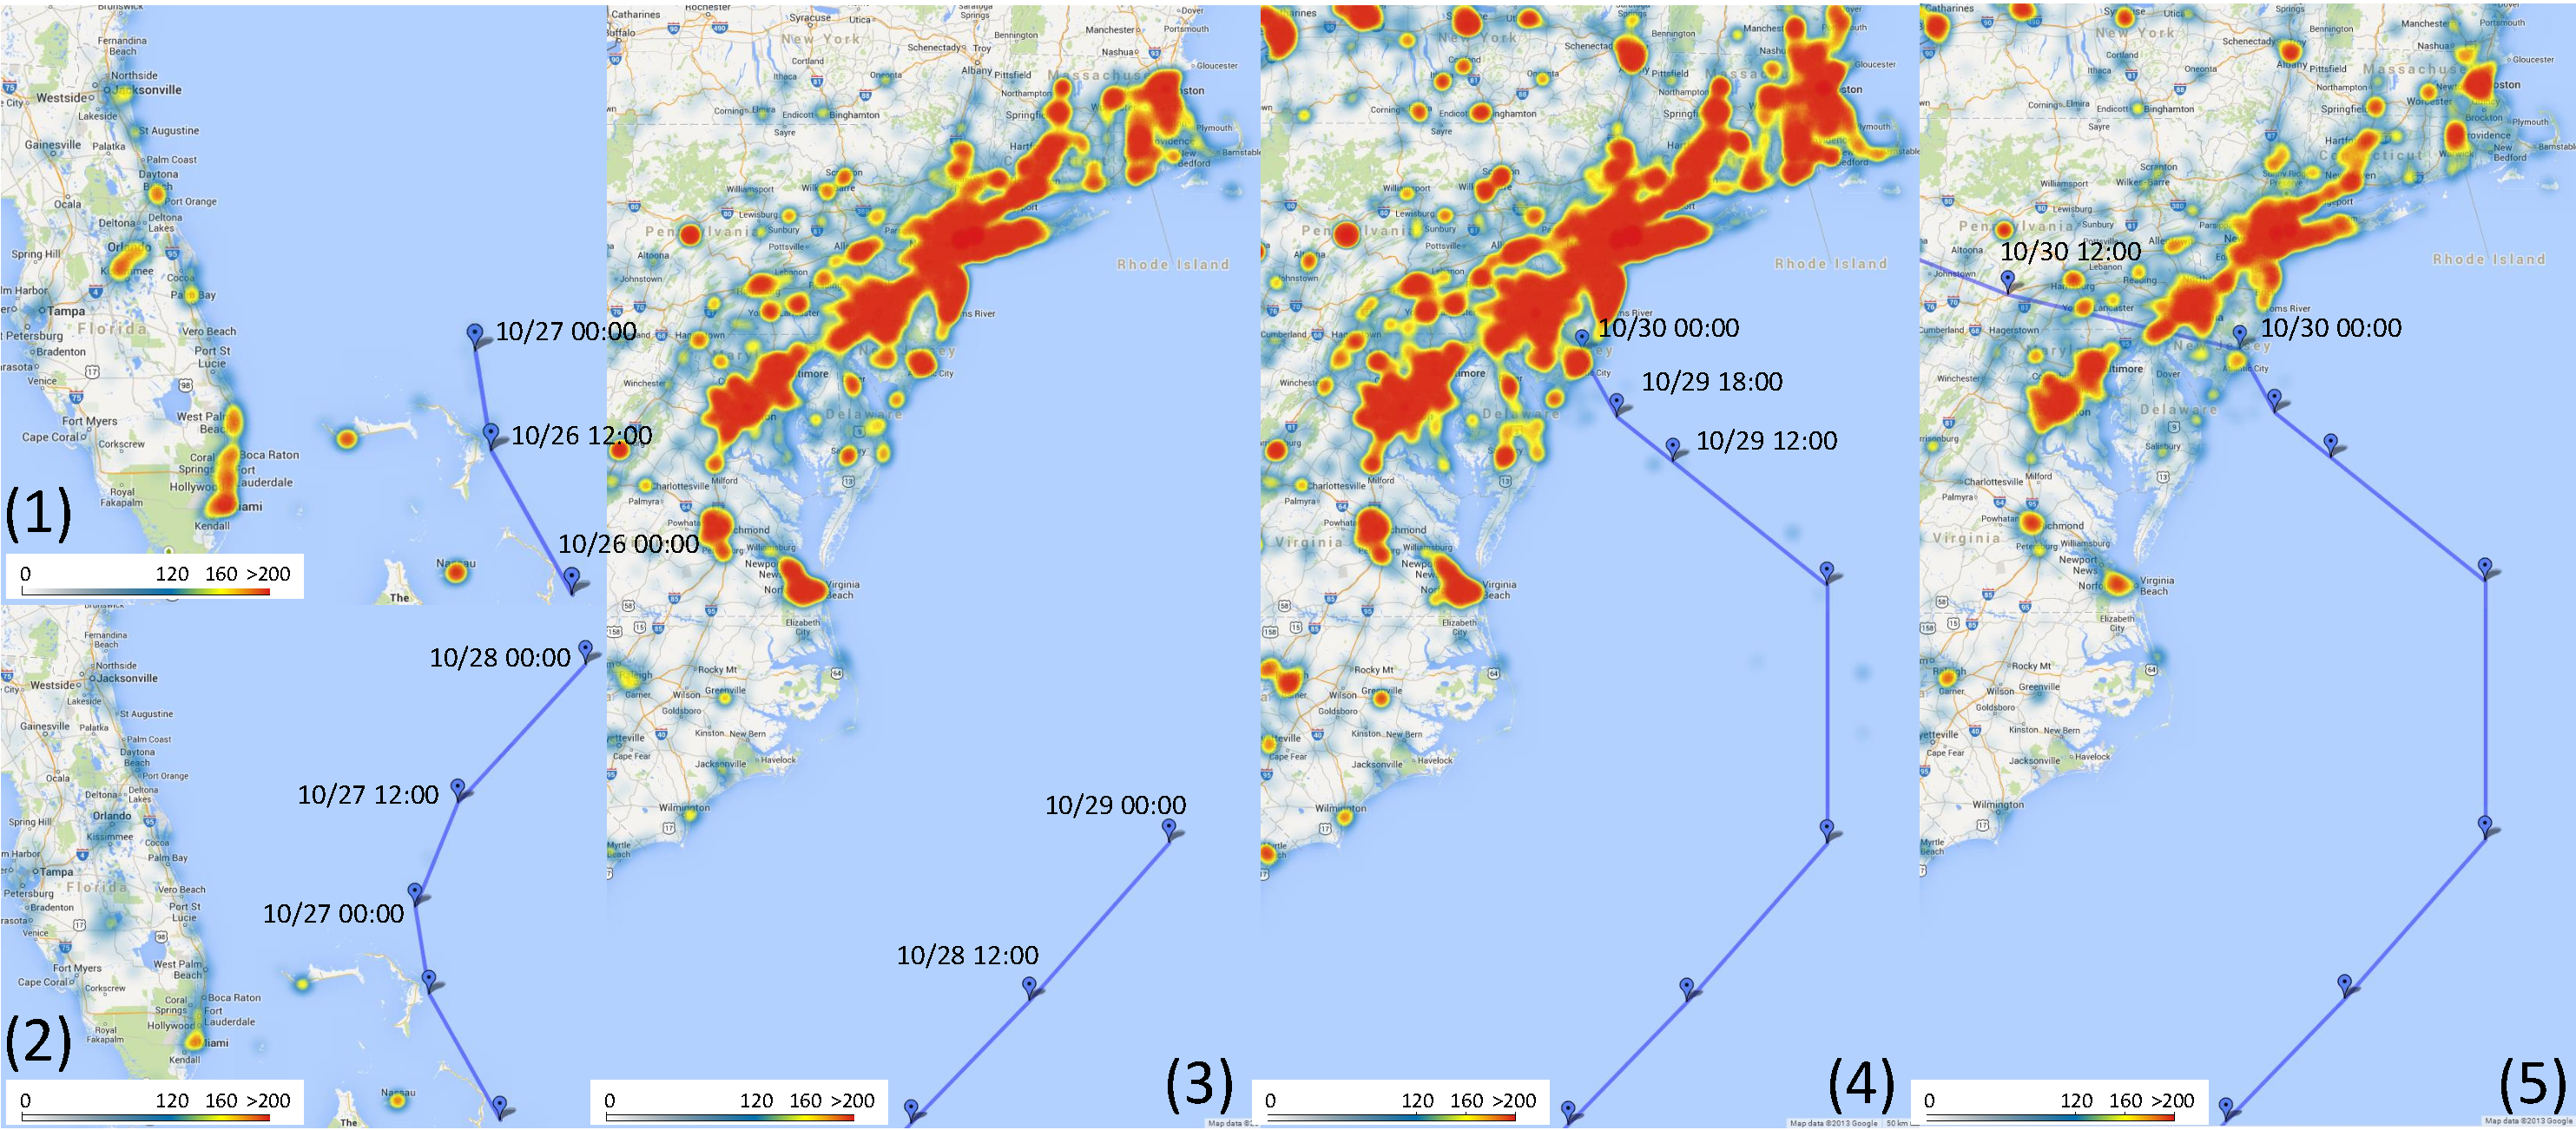
\includegraphics[width=1.0\linewidth]{East_Coast_v7}
\caption{Distribution of Twitter users of each consecutive date (Oct. 26 $\sim$ 30, 2012), who post hurricane related Tweets on the southeastern (1 and 2) and northeastern coast (3, 4, and 5) area of the United States. We can see the variance of Twitter user reactions along the track of the hurricane center locations.}
\label{fig:east_coast}
%\vspace{-0.4cm}
\end{figure}

Twitter users also actively respond to the severe weather conditions.
In Figure~\ref{fig:east_coast}, we indicate that the distribution pattern of Twitter users had dynamically varied along the track of the hurricane center locations.
When Sandy moved to the southeastern coast on October 26th, there were bursts on eastern Florida's coast (Figure~\ref{fig:east_coast}~(1)).
Next day, the bursts disappeared, because Sandy moved towards the northeast away from the east coast of United States (Figure~\ref{fig:east_coast}~(2)).
Sandy kept moving towards a few hundred miles southeast of North Carolina on October 28th (Figure~\ref{fig:east_coast}~(3)).
In the next day, the hurricane's track bent towards the north and the hurricane made landfall at night in the northeast of Atlantic City 
(Figure~\ref{fig:east_coast}~(4)).
Throughout the days, Twitter users were actively reacting to Hurricane Sandy' arrival in a wide range of areas.
After the landfall, the storm turned toward the northwest and was gradually weakened.
The big outbreaks were diminished on October 30th as shown in Figure~\ref{fig:east_coast}~(5).
As shown in the figures, we can see how Twitter users reacted according to the spatiotemporal pattern of the severe weather conditions in the social media domain.
%The Twitter user distributions along the track of the hurricane helps the users to understand the situations and further analysis.

%\textbf{Damage Area along the Tornado's Path:} 
\textbf{Damage Area from a Tornado:} An extremely strong Tornado passed through the city of Moore in southern metropolitan Oklahoma City~\cite{WKP:2013:MOORE} in the afternoon on May 20th, 2013.
The larger than one-mile-wide tornado damaged the city with a wind speed of more than 200~mph.
Figure~\ref{fig:tornado} shows the damaged part of the city.
The tornado entered the area at about 3:16 PM and exited the area after about 10 minutes.
We visualize the distribution of Twitter users on the map during 24 hours, from May 20th 4:00 PM to 21st 4:00 PM.
%This result represents the situation after the city was severely damaged by the tornado.
We also overlay an approximate extent of tornado damage (transparent orange color) and locations of multiple infrastructures, such as schools, hospitals, and supermarkets, on the map view.
Since the tornado suddenly happened and disappeared, we were not able to find significantly abnormal patterns before and during the event. 
%In Section~\ref{sec:discussion}, we will discuss about this in detail.
After the disaster event, however, many Twitter users moved toward some specific areas: two elementary schools, a medical center, a theater, and two large supermarkets.
The two elementary schools, the medical center, and the theater were located within the highly damaged area and they were severely destroyed.
Also many people were hurt and died in these infrastructures.
The increased number of Twitter users was probably due to the fact that many people went to these places in order to rescue the victims~\cite{TWITCHY:2013:CHG}.
Moreover, people might have gone to supermarkets to obtain indispensable things.
In Figure~\ref{fig:tornado}~(1), the heatmap shows a normal situation of Twitter user distribution in the same area.
The distribution is very different from the situation after the tornado hit the area.
This example demonstrates how our visual analytics system enables the analysts to analyze public responses using spatial disaster data and infrastructure data for disaster management.

\begin{figure}[tbh]
\centering
%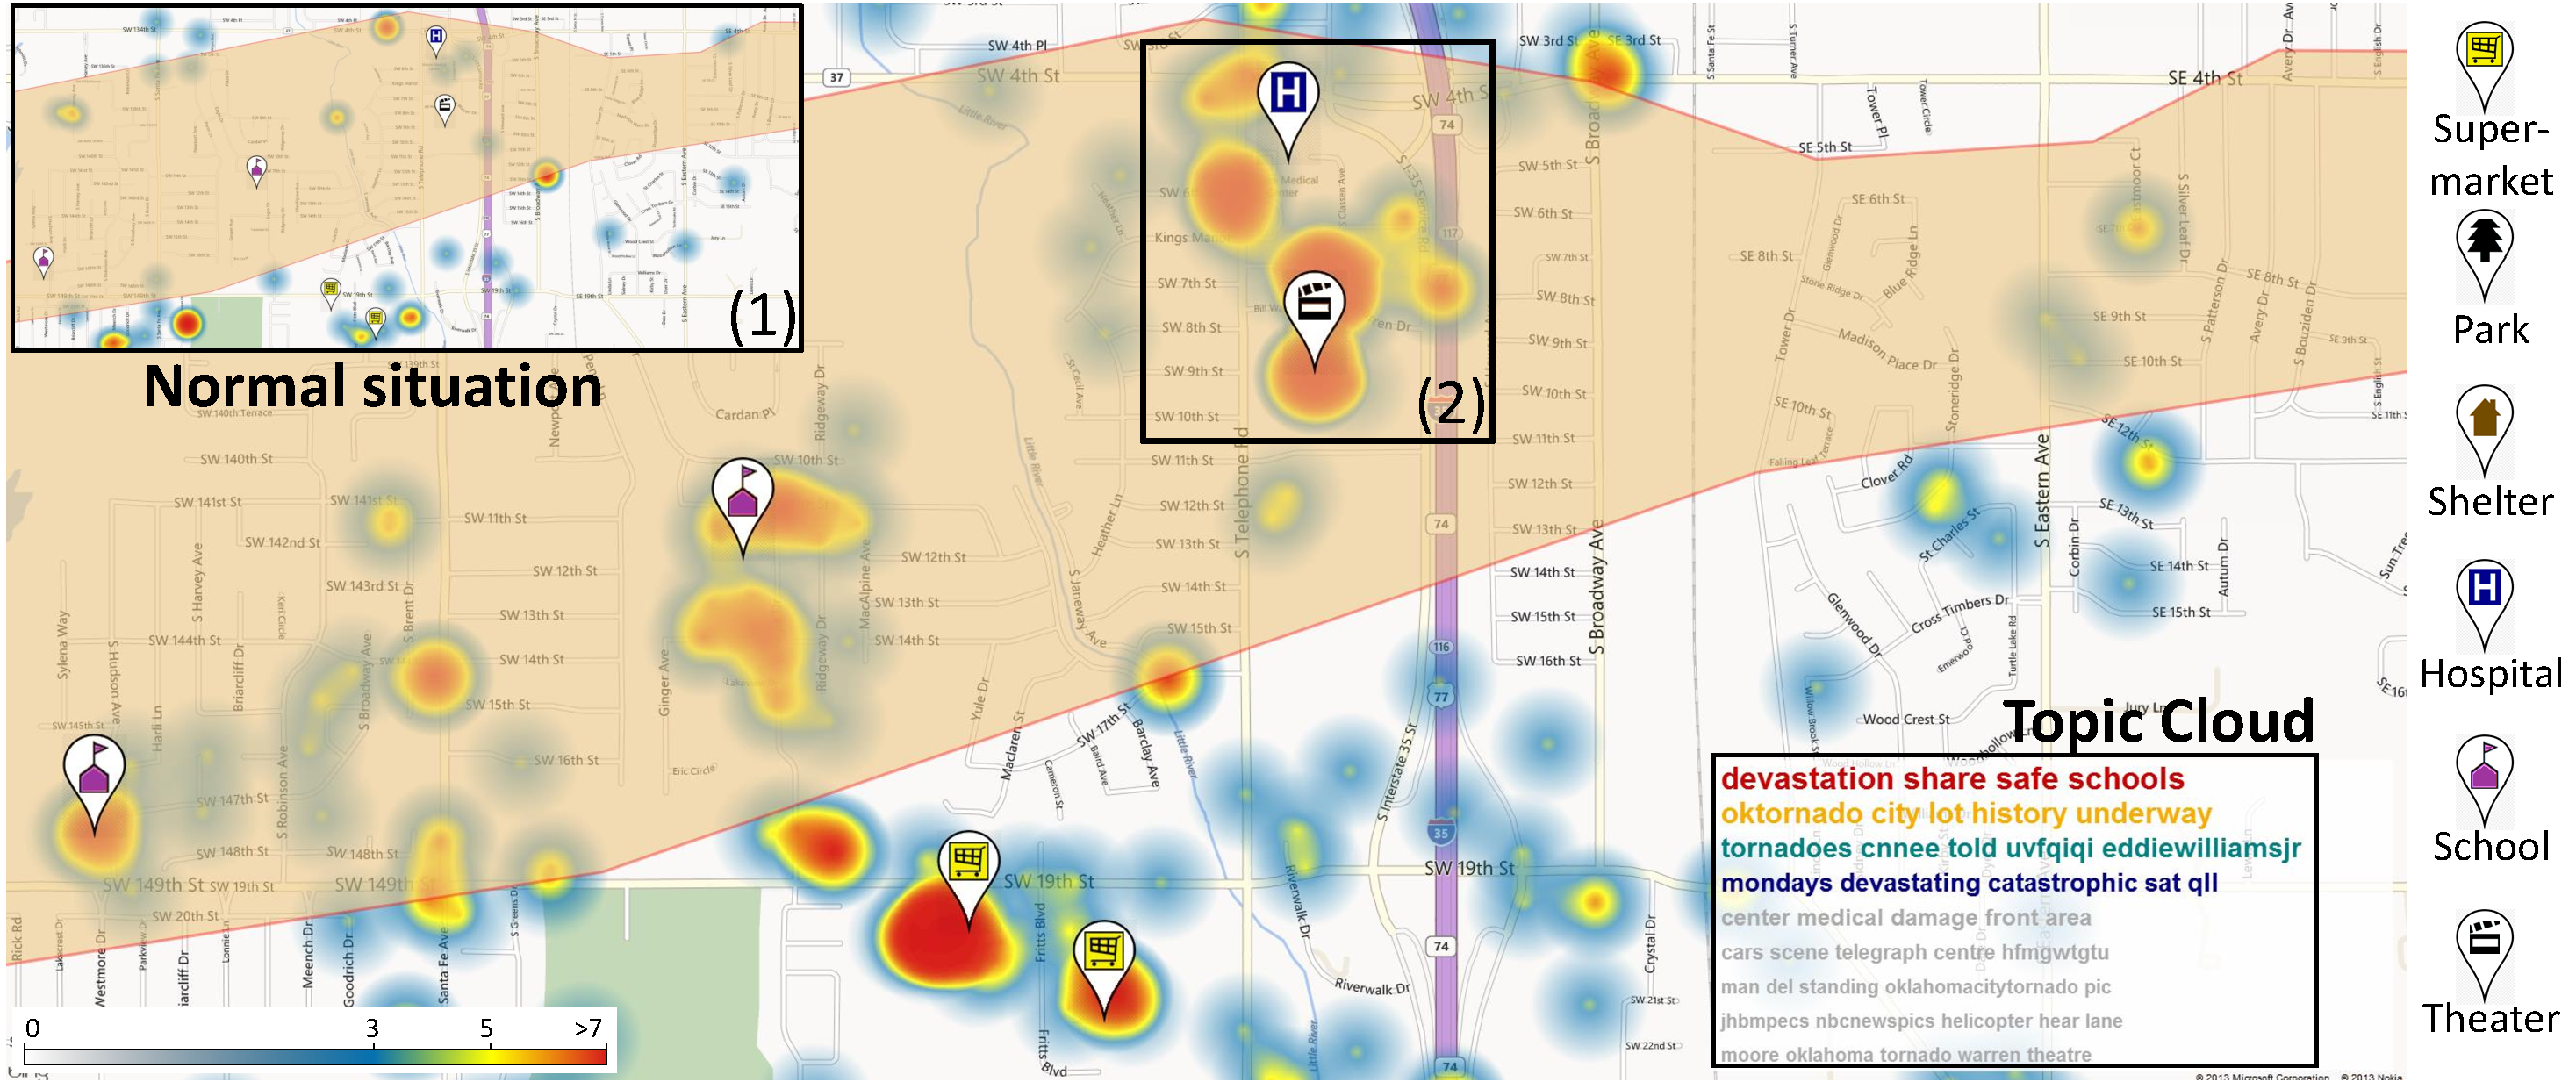
\includegraphics[width=0.9\linewidth]{Tornado_v9}
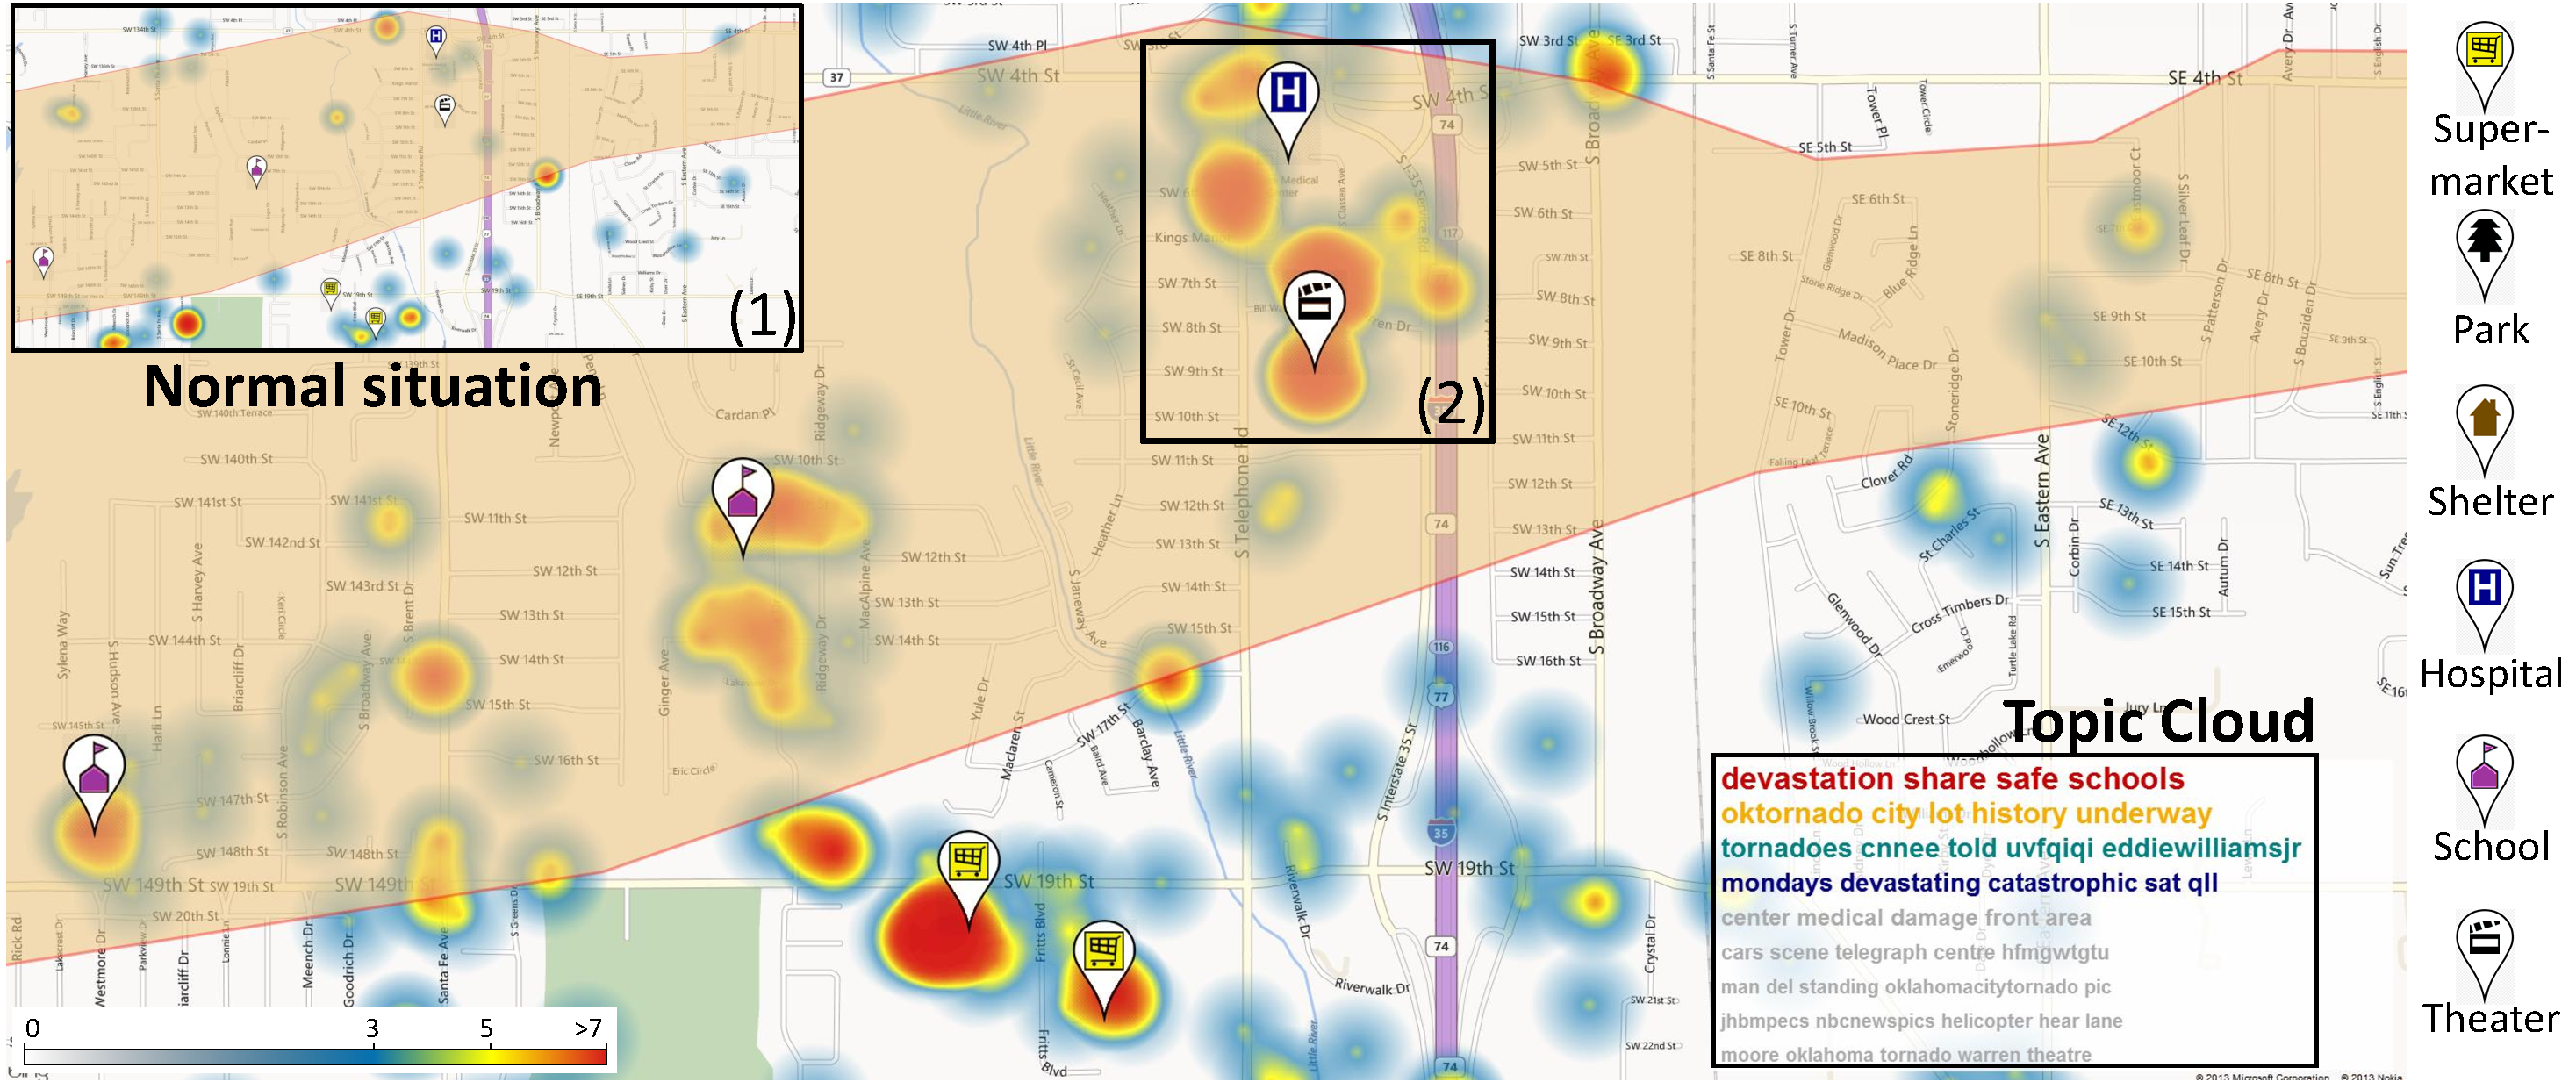
\includegraphics[width=1.0\linewidth]{Tornado_v9}
\caption{Spatial pattern of Twitter users during 24 hours in the city of Moore after damages from a strong tornado. Relatively many people moved to severely damaged areas after the disaster. This situation is much different from the previous normal situation (1). We selected a specific region (2) that includes severely damaged areas in order to extract topics (3) from Tweets within the selected area.}
\label{fig:tornado}
%\vspace{-0.2cm}
\end{figure}

\subsubsection{Abnormal Topic Analysis}
\label{sec:abnormal_topic_analysis}
\begin{figure}[tb]
\centering
%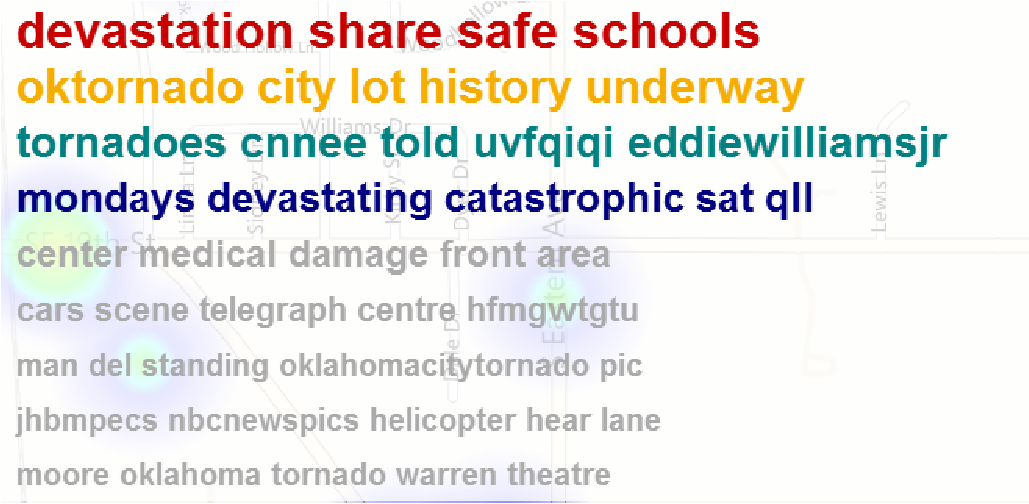
\includegraphics[width=0.85\columnwidth]{Topiccloud_v2}
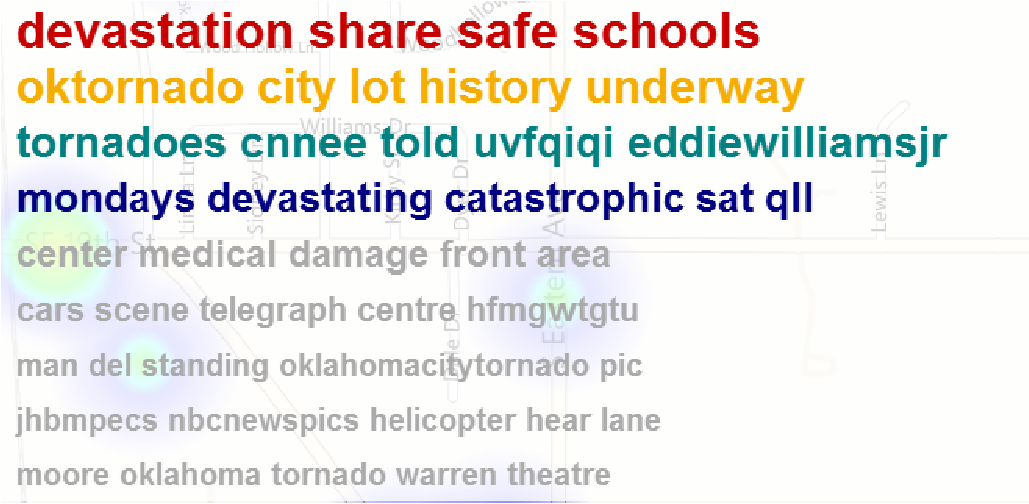
\includegraphics[width=0.8\linewidth]{Topiccloud_v2}
\caption{Topic cloud: Topics from Tweets within the selected area in Figure~\ref{fig:tornado}~(2) are ordered by their abnormality scores.}
\label{fig:topic_cloud}
%\vspace{-0.4cm}
\end{figure}

Our system also provides analysts with abnormal topic examination within the microblog data.
Each Twitter message provides not only spatiotemporal properties, but also textual contents.
The text messages are also important to understand and examine the emergent situations.
Our system allows the analysts to extract major topics from many Tweets posted within a specific area using the LDA~\cite{Blei:2003:LDA}.
We also employ, then, the STL~\cite{Cleveland:1990:SAS} to identify unusual topics within the selected area.
For each extracted topic of the LDA topic modeling, our algorithm retrieves messages associated with the topic and then generates a time series consisting of daily message counts from their timestamps.
The time series can be considered as the sum of three components: a trend component, a seasonal component, and a remainder.
Under normal conditions, the remainder will be identically distributed Gaussian white noise, while a large value of the remainder indicates substantial variation in the time series.
Thus, we can utilize the remainder values to implement control chart methods detecting anomalous outliers within the topic time series.
We have chosen to utilize a seven day moving average of the remainder values to calculate the z-scores.
Note that we use the z-score as the abnormality score in this work.
If the z-score is higher than 2, events can be considered as abnormal within a 95\% confidence interval.
The details of these techniques are described in the previous work~\cite{CHAE:2012:SSM}.
We select a sub area in Figure~\ref{fig:tornado}~(2) that includes severely damaged areas: the selected region (black rectangle) on the map.
The extracted topics, which are ordered based on their abnormalities, are displayed as Topic Clouds at the bottom-right corner (Figure~\ref{fig:tornado}~(3)) on the map.
The topic cloud is enlarged and shown in Figure~\ref{fig:topic_cloud}.
In this case study, most topics are related to the disaster event. 
However, the last topic\textemdash \textit{moore, oklahoma, tornado, warren, theatre}, has a relatively low abnormality although they seem related to the disaster event, because tornadoes frequently occur in the area.
%Our abnormal topic analysis enables the analysts to understand what situations are going within the area.
Figure~\ref{fig:abnormality_graph} shows an abnormality graph for the first topic in Figure~\ref{fig:topic_cloud}.
The abnormality score for the topic had significantly increased when the tornado hit the region on May
20th (Marked region). As shown in Figure~\ref{fig:abnormality_graph}, the abnormality score (6.75) is much higher than the average abnormality score(0.42); therefore, the analysis of the microblog data provides a statistically significant difference during this severe weather condition.



\begin{figure}[tb]
\centering
%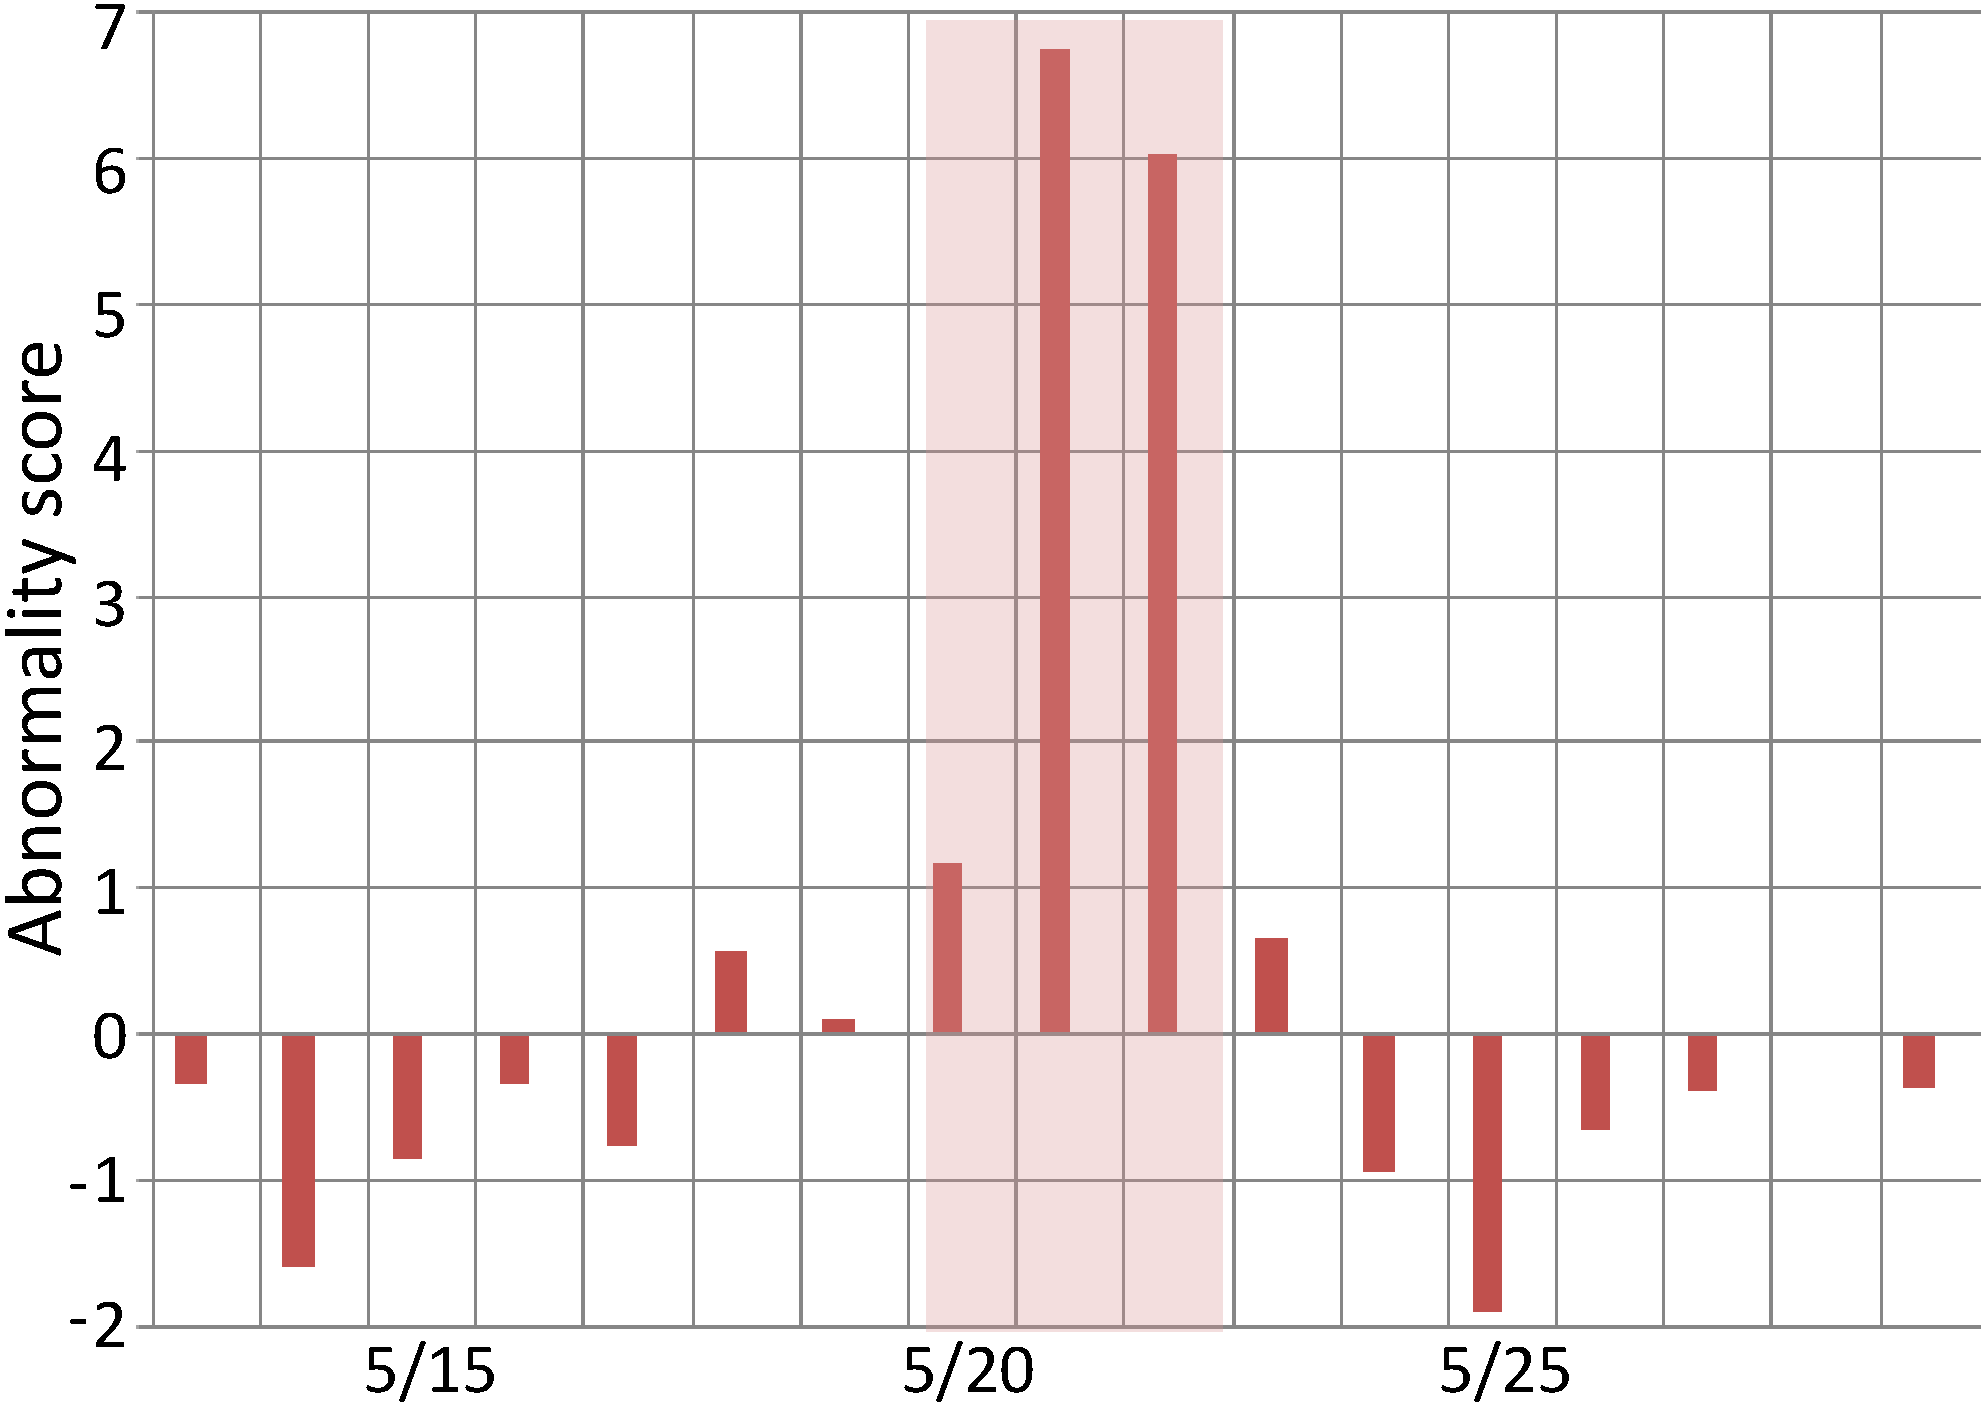
\includegraphics[width=0.7\columnwidth]{Topiccloud_zscore_graph_v3}
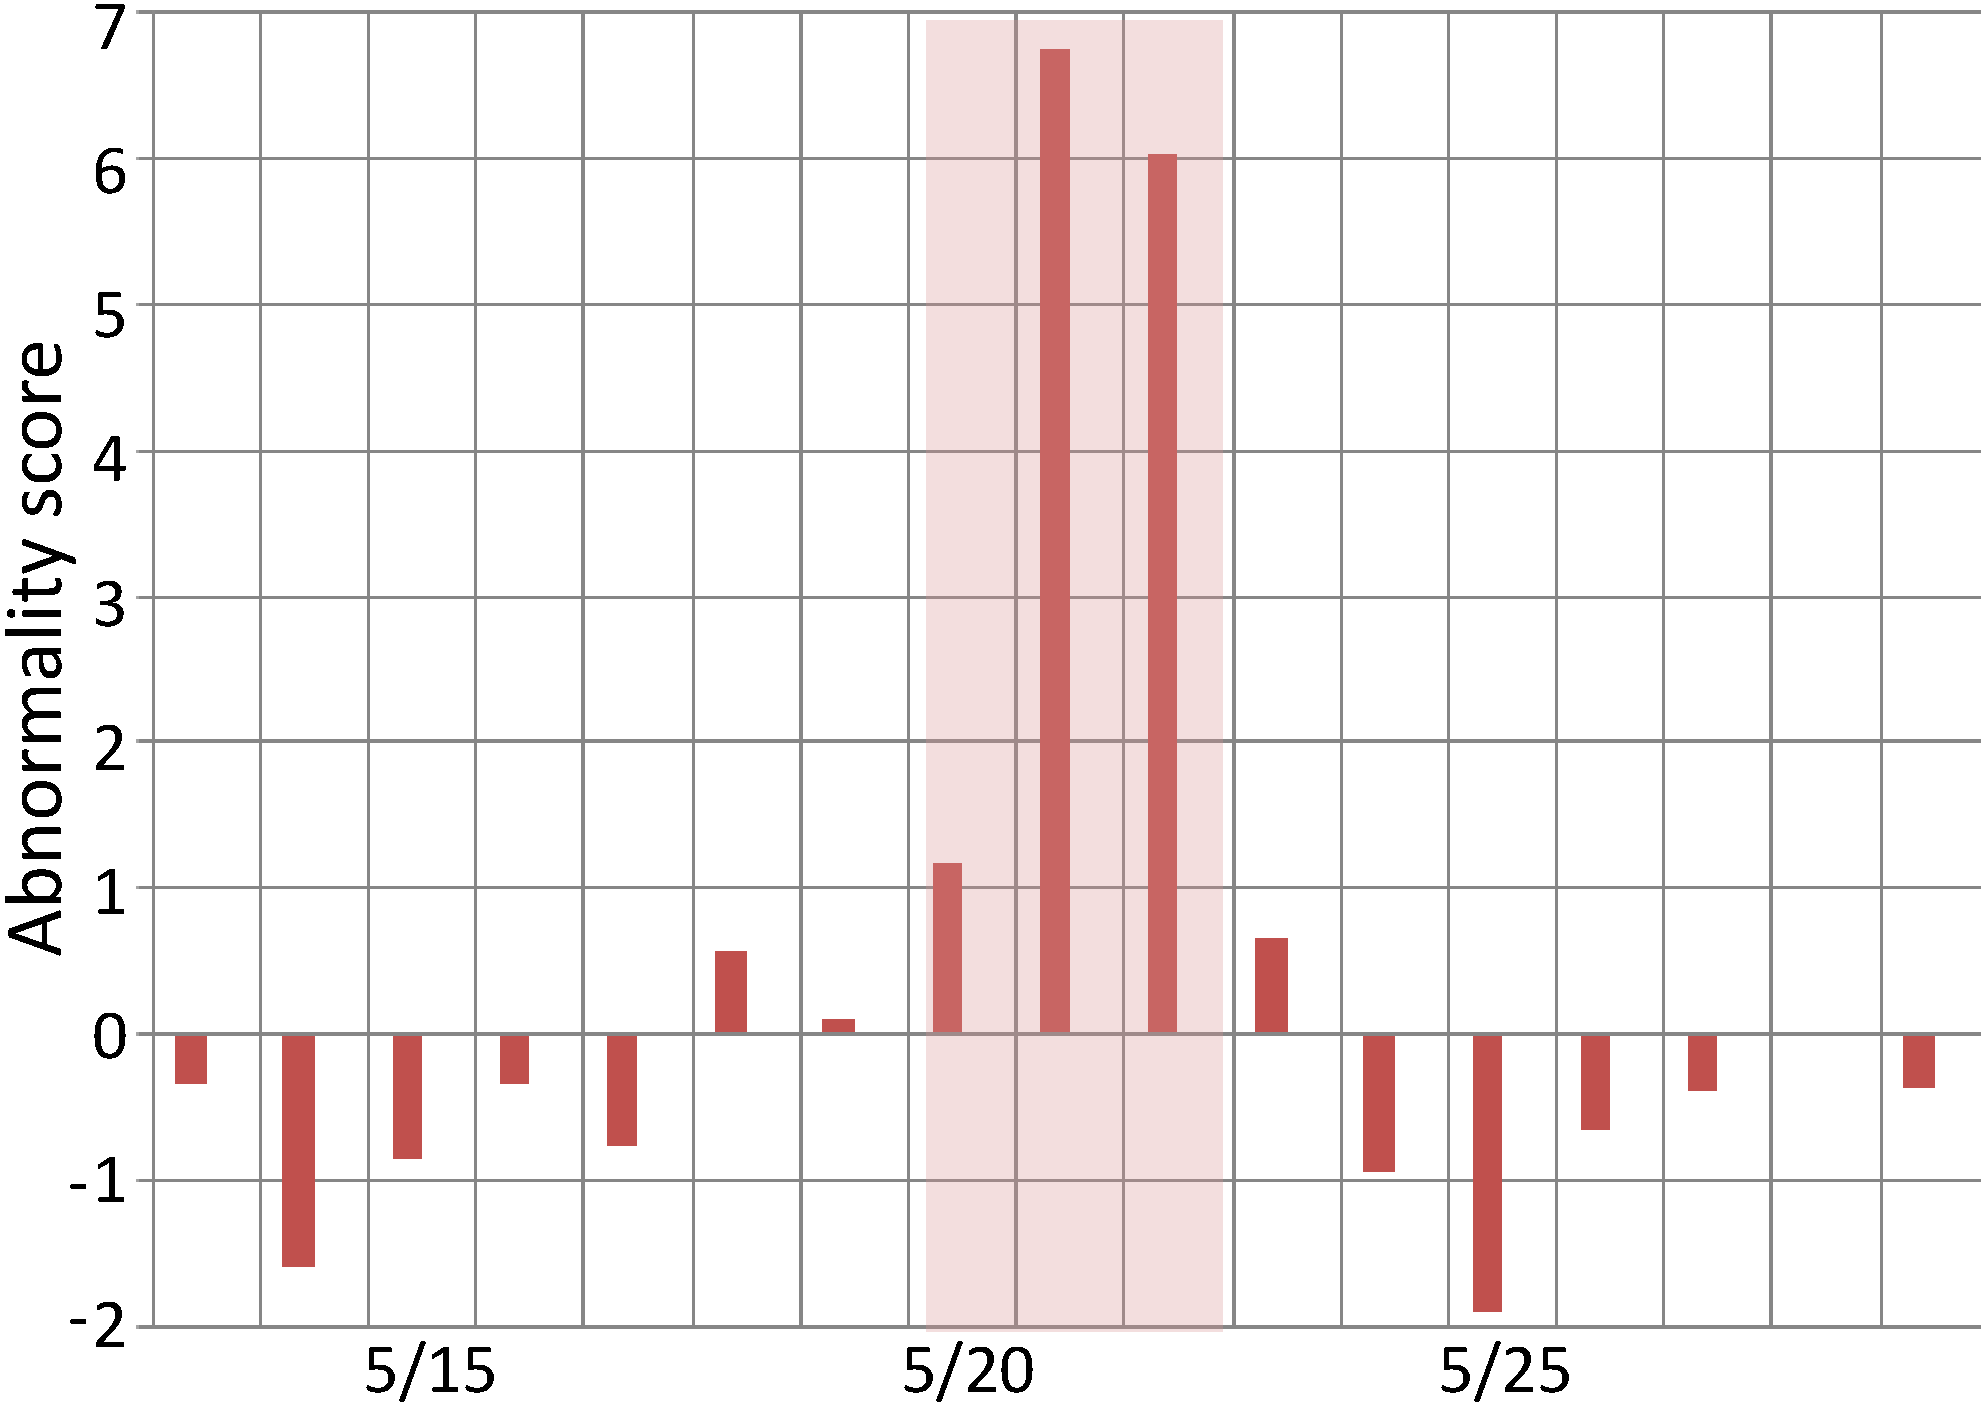
\includegraphics[width=0.8\linewidth]{Topiccloud_zscore_graph_v3}
\caption{Abnormality of the first topic in Figure~\ref{fig:topic_cloud}. 
The abnormality score of the topic had significantly increased when the tornado hit the region on May 20th (Marked region).}
\label{fig:abnormality_graph}
%\vspace{-0.4cm}
\end{figure}


\subsection{Temporal Pattern Analysis}
\label{sec:temporal_pattern}
%
%Describe the graph
%In Section~\ref{sec:spatial_analysis}, we present spatial analysis of social media and spatial decision support using multiple types of supplementary data in order to reveal where and why a number of people move.
In the previous sections, we presented the spatial analysis of social media and spatial decision support. 
In this section, we demonstrate analysis of the relationships between the temporal patterns of the number of Twitter users and certain public situational behaviors:
%using time-stamp information of Tweets
how many people go where and how different is it from previous situations?
Analysis of temporal trends and relationships between data values across space and time provides underlying insights and improves situational awareness~\cite{Maciejewski:2010:FHP, Malik:2011:DTC}.


After selecting the initial spatiotemporal context of Tweets as a basis for the analysis, the analysts can explore the temporal patterns of the number of Twitter users who posted Tweets within the spatial boundary using the bar chart as shown in Figure~\ref{fig:graph}.
The values of each bar are the number of users in four hour intervals and represent data two weeks before and after the selected date.
Once a mouse cursor hovers over one of the bars in the graph, every bar that corresponds to that time period, is highlighted in dark yellow color as shown in Figure~\ref{fig:graph}.
As previously mentioned, the heatmap in the figure shows the Twitter user density distribution from 12:00 PM to 4:00 PM on October 28th, right after the announcement of the evacuation order.
We select a hotspot that includes one of the supermarket locations: the selected region (black rectangle) on the map in Figure~\ref{fig:heatmap_manhattan} (Right).
We can indicate that the number of Twitter users (red rectangle in Figure~\ref{fig:graph}) in the corresponding time period is higher than for the same time period from other dates (October 14th, 21st and November 4th, 5th) by 35\% more from the average.
Moreover, there is another interesting finding\textemdash the number of people during each of the following time frame (4:00 $\sim$ 8:00 PM) on the dates from the previous weeks are higher than the number of people in the selected time frame.
This is because many shoppers were lining up at stores and emptied the shelves to prepare for Hurricane Sandy.
Some actual Twitter messages posted in the area are following: \textit{\textquoteleft The line at Trader Joes is unbelievable ...\textquoteright} and \textit{\textquoteleft There is amazing line here ...\textquoteright}.
Furthermore, since October 29th, the number of people has significantly decreased because most residents left the area before the arrival of the hurricane.
The increase in the number of people after one week reflects that some people came back to the area.
% and even shows when the stores reopened.

%Social media use rises during disasters as people seek immediate and in-depth information%~\cite{STAR}.
%reflect that the number users increased during sandy, but the situation had been gone since evacuation or severe damage for example, power outage caused by flooding and strong wind.

\begin{figure}[tbh]
\centering
%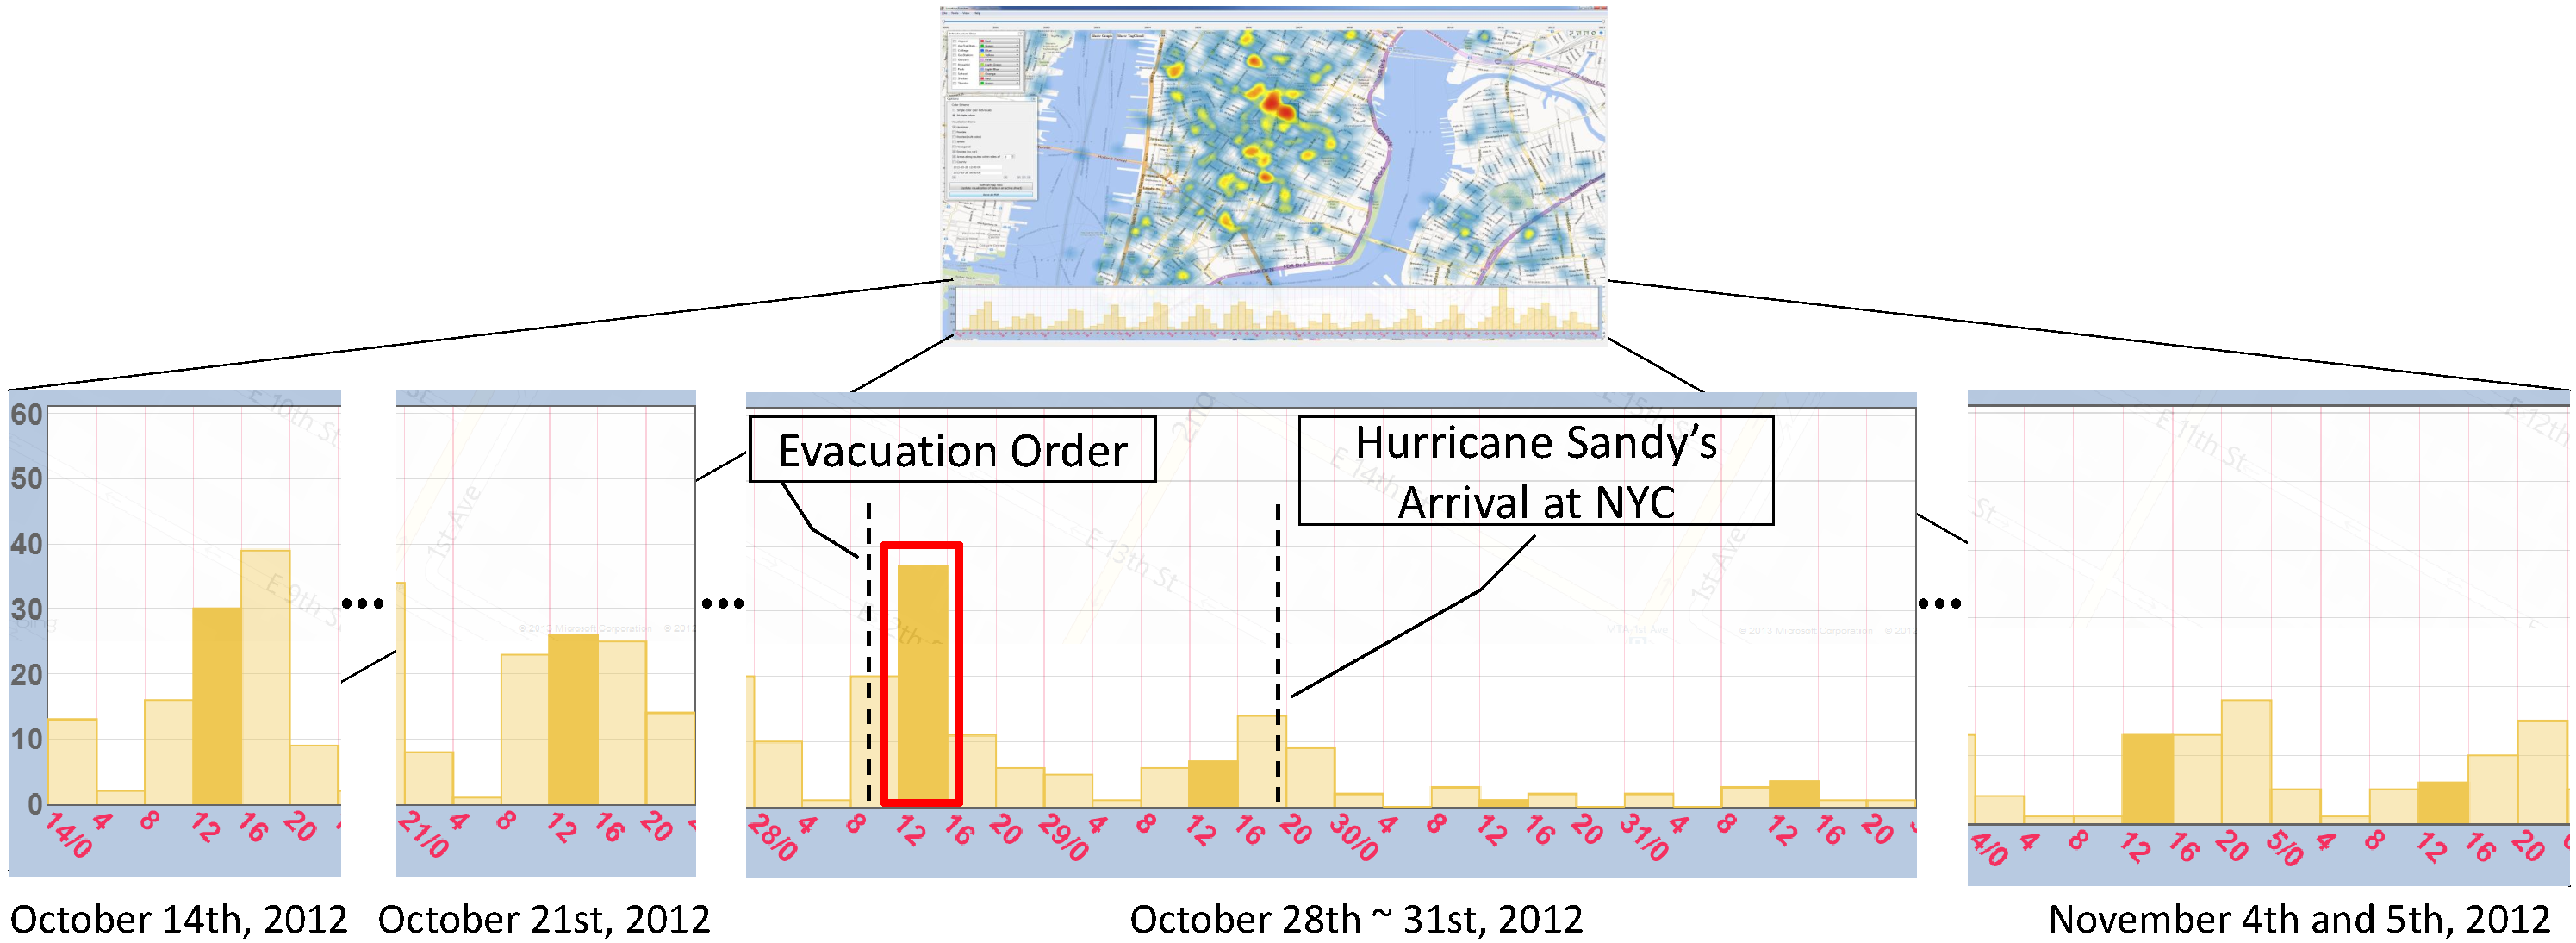
\includegraphics[width=0.80\linewidth]{graph_system_v4}
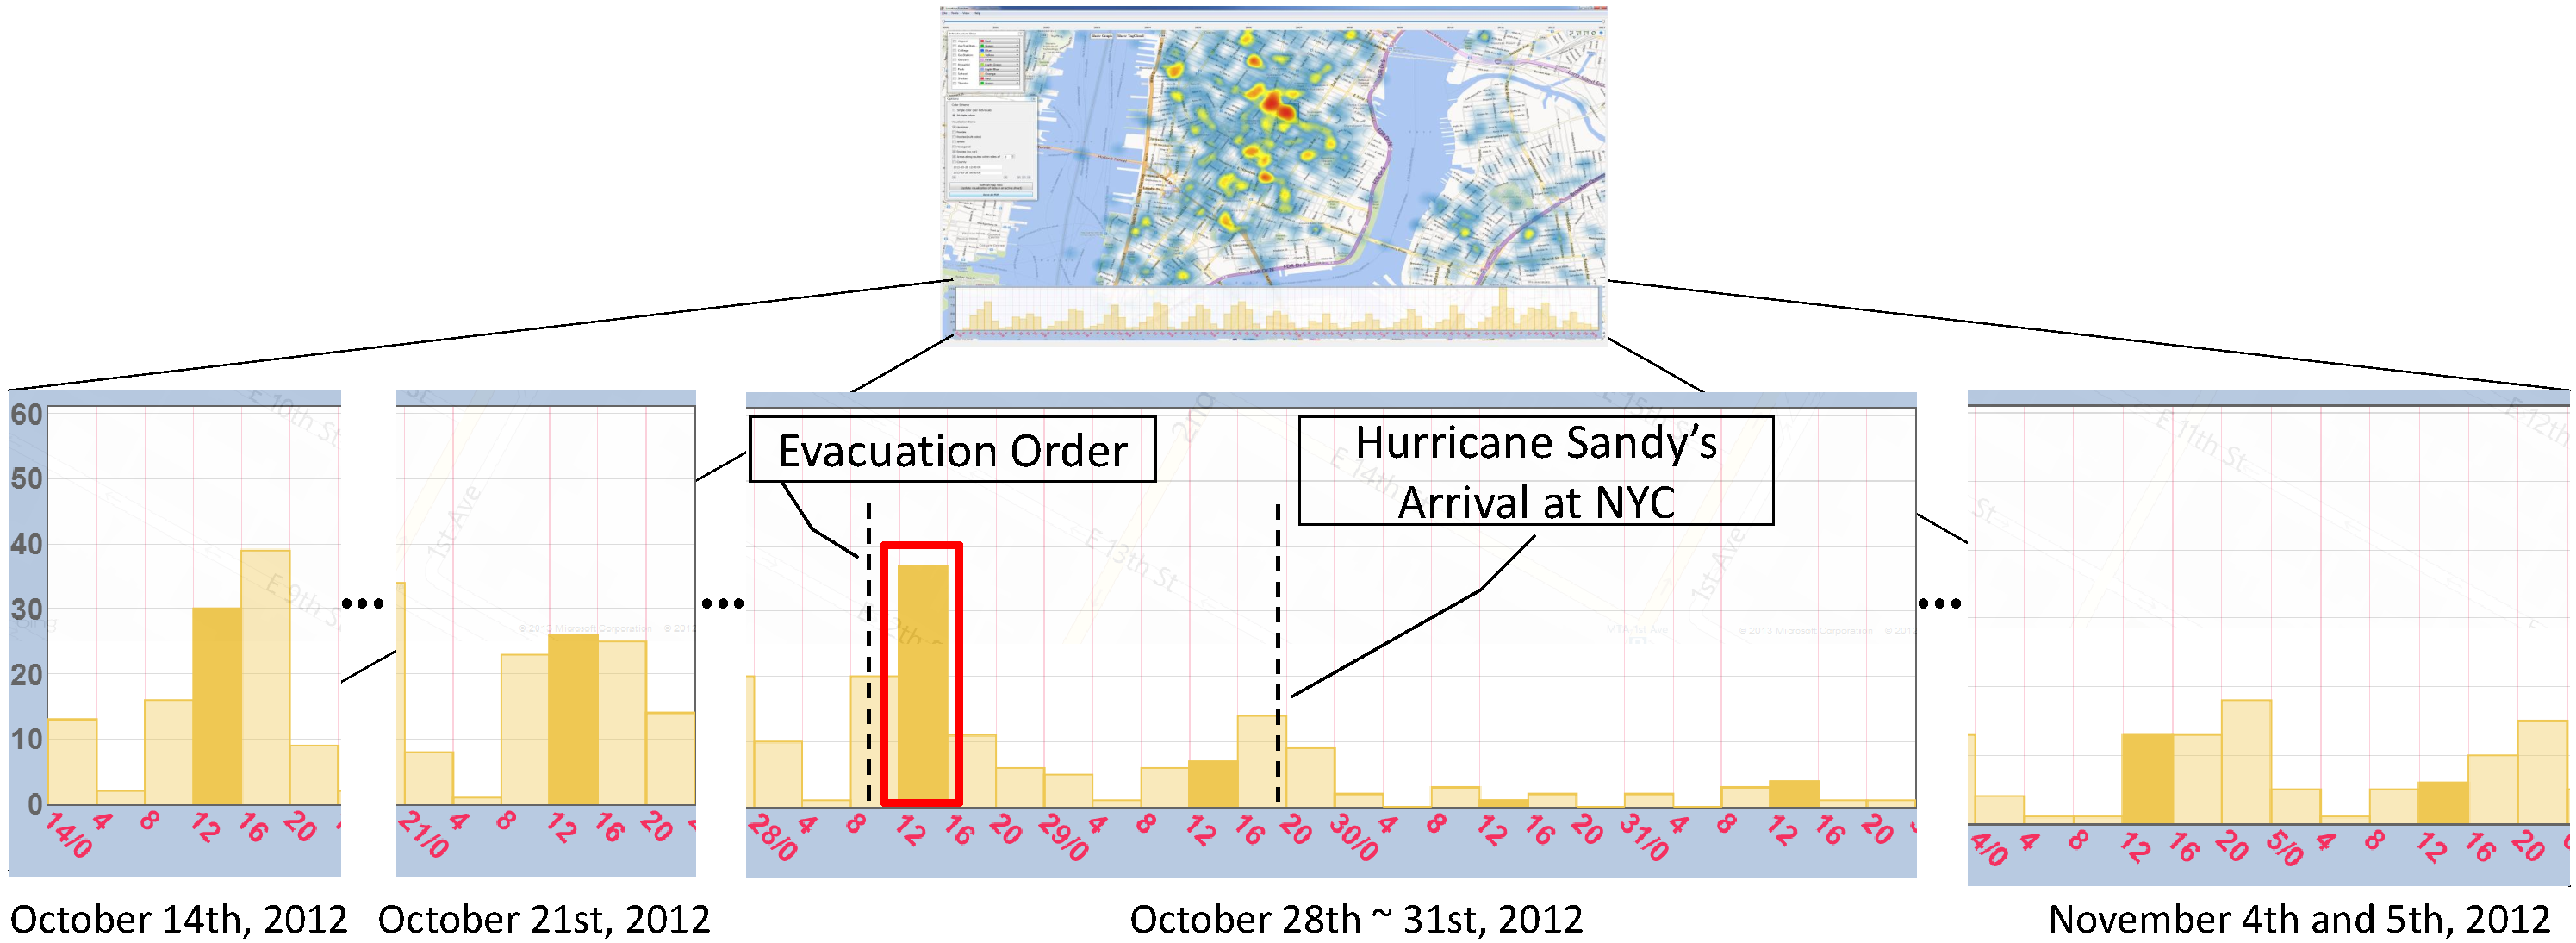
\includegraphics[width=1.0\linewidth]{graph_system_v4}
\caption{Temporal analysis for public behaviors during the disaster event, Sandy. Top shows our entire system view. 
The bar chart (Bottom) for the number of Twitter users within the selected region including a supermarket in Figure~\ref{fig:heatmap_manhattan} (Right) in four hour intervals is shown.
%some interesting time frames of the entire plot on the system. 
We see that many people went to the supermarket right after the evacuation order.}
\label{fig:graph}
%\vspace{-0.4cm}
\end{figure}




